\section{Experiments and Analysis}
\label{sec:experiments}

\paragraph{Overview.}
We conduct a series of experiments to identify the capabilities and limitations of modern VLMs on \textsc{ViTALBench}. Our analysis is organized around four research area questions:

\begin{itemize}
\item \textbf{RQ1.} How does model performance change as questions move from visual scene understanding to increasingly statute-dependent legal reasoning?

\item \textbf{RQ2.} To what extent can statutory evidence close the
performance gap between perception and legal reasoning?

\item \textbf{RQ3.} Are models aware of their own knowledge gaps, abstaining
more when a question requires statutory grounding?
\item \textbf{RQ4.} How does model capacity affect the ability to leverage supplied statutory evidence?

\end{itemize}


\subsection{Experimental Setting}

\paragraph{Dataset.}
We conduct experiments on \textsc{ViTALBench} to evaluate the visual and legal reasoning capabilities of current VLMs. \textsc{ViTALBench} comprises a detection tier (\textbf{Detection}; 2{,}122 items) and a legal tier (2{,}414 items) split by the reasoning it demands: \textbf{Violation Identification} (482), \textbf{Regulation Application} (1{,}601), and \textbf{Multi-step Legal Reasoning} (331). All legal questions are grounded in current Vietnamese traffic regulations.

\paragraph{Models.}
We evaluate ten open VLMs from four model families and across a broad range of parameter scales. These include InternVL3 \cite{zhu2025internvl3exploringadvancedtraining} with 1B, 2B, 8B, and 14B parameters, Qwen3-VL-Instruct \cite{bai2025qwen3vltechnicalreport} with 2B, 4B, and 8B parameters, Qwen2.5-VL \cite{bai2025qwen25vltechnicalreport} with 3B and 7B parameters, and Llama-3.2-11B-Vision \cite{touvron2023llamaopenefficientfoundation}.

\paragraph{Configuration and metrics.}
All models are evaluated in BF16 on a single NVIDIA A100 40 GB GPU using identical prompts and inference settings. We report multiple-choice accuracy under two evaluation protocols. The 4-option protocol contains only the four candidate answers, whereas the 5-option protocol adds an explicit \textit{Not sure} option, allowing models to abstain rather than select one of the content answers.

% ============================================================
\section{Analysis Results}
\label{sec:results}

% ------------------------------------------------------------
\subsection{A large gap separates perception from legal reasoning}
\label{sec:gap}
\paragraph{Experiments.} To examine how performance changes as questions progress from visual scene understanding to increasingly statute-dependent legal reasoning, all ten VLMs are evaluated under the 4-option protocol. Accuracy is reported in Table~\ref{tab:pertype} separately for Perception, Violation Identification, Regulation Application, and Multi-step Legal Reasoning. The average across the three legal categories is also reported as the overall legal-tier accuracy.
\paragraph{Analysis.}
All ten models perform substantially better on Perception than on the legal tier. Across models, average accuracy falls from $83.5\%$ on Perception to $60.1\%$ on legal questions, producing a consistent gap of $23.4$ percentage points. This gap shows that strong visual understanding does not necessarily translate into legally grounded decisions.

Performance generally declines as questions become more dependent on statutory knowledge. Average accuracy decreases from $68.7\%$ on Violation Identification to $58.9\%$ on Regulation Application and $53.3\%$ on Multi-step Legal Reasoning. Models can often identify a violation from visible behavior, but they struggle when required to determine the governing provision, apply relevant legal conditions, and infer the corresponding consequences. The main difficulty, therefore, emerges when models must move beyond recognizing a traffic event and ground their decisions in specific legal rules. Increasing model size does not consistently close this gap. Within InternVL3, scaling from 1B to 14B reduces the gap between Perception and Violation Identification from $19.1$ to $1.9$ points, while increasing the gap between Perception and Regulation Application from $15.8$ to $29.3$ points. Qwen3-VL shows a similar pattern from 2B to 8B, with Violation Identification improving by $15.1$ points but Regulation Application by only $7.9$ points. Overall, scaling substantially improves visual understanding and violation recognition, but does not reliably improve the ability to interpret and apply the relevant law.

\begin{table}[t]
\centering
\caption{Accuracy (\%) by question type (4-option protocol). Every model is far stronger on Perception than on the legal tier, and within the legal tier, it drops most in Regulation Application and Multi-step Reasoning. Column maxima in bold. $^{\dagger}$Item-weighted average over the three legal types.}
\label{tab:pertype}
\setlength{\tabcolsep}{6pt}
\begin{tabular}{lccccc}
\toprule
Model & Perception & Vio.\,ID & Reg.\,App & Multi & Legal$^{\dagger}$ \\
& $\uparrow$ & $\uparrow$ & $\uparrow$ & $\uparrow$ & $\uparrow$ \\
\midrule
InternVL3-1B  & 74.3 & 55.2 & 58.5 & 53.8 & 57.2 \\
InternVL3-2B  & 80.9 & 49.6 & 53.3 & 45.3 & 51.5 \\
InternVL3-8B  & 89.2 & 80.1 & 63.5 & 60.7 & 66.4 \\
InternVL3-14B & \textbf{91.3} & \textbf{89.4} & 62.0 & 61.9 & 67.4 \\
Qwen3-VL-2B   & 81.6 & 64.9 & 55.9 & 45.3 & 56.3 \\
Qwen3-VL-4B   & 88.1 & 82.0 & 59.8 & 59.2 & 64.2 \\
Qwen3-VL-8B   & 89.6 & 80.1 & \textbf{63.8} & \textbf{62.5} & 66.9 \\
Qwen2.5-VL-3B & 81.7 & 73.9 & 54.5 & 49.2 & 57.7 \\
Qwen2.5-VL-7B & 85.4 & 67.2 & 56.6 & 49.8 & 57.8 \\
Llama-3.2-11B & 72.9 & 45.0 & 61.4 & 44.7 & 55.8 \\
\midrule
Average
& 83.5
& 68.7
& 58.9
& 53.3
& 60.1 \\
\bottomrule
\end{tabular}
\end{table}

% ------------------------------------------------------------
\subsection{Gold statutory evidence recovers much of the legal performance gap}
\label{sec:oracle}

\paragraph{Experiments.}
We examine whether the lower legal-tier performance is primarily associated with limited access to the governing law. For each legal question, we provide the model with the gold statutory provision at inference time and evaluate it under the \textsc{Legal}$_{+\text{gold}}$ setting. We compare this result with the original legal-tier accuracy obtained without external evidence. The Figure~\ref{fig:gold} presents the comparison for all ten models.


\paragraph{Analysis.}
Providing the governing provision improves legal accuracy for every model. The average gain is $14.2$ percentage points, with improvements ranging from $2.9$ points for InternVL3-1B to $18.8$ points for InternVL3-14B. InternVL3-14B improves from $67.4\%$ to $86.2\%$, while Qwen3-VL-8B increases from $66.9\%$ to $85.5\%$. Qwen3-VL-4B and Qwen2.5-VL-7B also show substantial gains of $18.0$ and $18.2$ points, respectively.

\begin{figure}[t]
\centering
    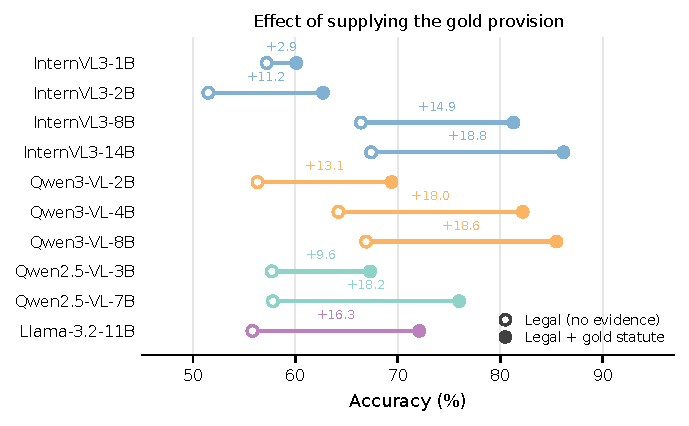
\includegraphics[width=\linewidth]{Figures/fig_gold_evidence.pdf}
\caption{Effect of supplying the governing statutory provision at inference.}
\label{fig:gold}
\end{figure}
The magnitude of improvement varies considerably across models. InternVL3-1B gains only $2.9$ points, whereas the larger InternVL3 models gain between $14.9$ and $18.8$ points. A similar pattern appears within Qwen3-VL, where the 2B model gains $13.1$ points but remains below the 4B
and 8B models after receiving the same gold evidence. These results indicate that limited access to statutory knowledge is a major source of error, but providing the correct provision does not guarantee successful legal reasoning. Models must still interpret the provision, connect its conditions to the visual evidence, and derive the appropriate legal consequence. The results, therefore,
highlight two complementary challenges: access to relevant statutory evidence and the ability to use that evidence effectively.



% ------------------------------------------------------------
\subsection{Abstention increases on statute-dependent questions}
\label{sec:abstain}
We next examine whether models express greater uncertainty when questions require statutory grounding. We extend the original 4-option protocol by adding a fifth option, \textit{Not sure}, allowing models to abstain rather than select one of the content answers. We measure the percentage of questions for which each model selects this option and report the results separately for Perception, Violation Identification, Regulation Application, and Multi-step Legal Reasoning in Table~\ref{tab:abstention}.


\paragraph{Analysis.}
Models abstain much more frequently on questions that require statutory knowledge. Across all models, the mean abstention rate is only $2.3\%$ for Perception and $3.8\%$ for Violation Identification. However, it increases to $25.0\%$ for Regulation Application and $21.9\%$ for Multi-step Legal Reasoning. Models, therefore, select \textit{Not sure} nearly eight times more often on the two statute-dependent categories than on the two categories that rely primarily on visual evidence.

This pattern is particularly clear for several models. InternVL3-14B abstains on only $2.1\%$ of Perception questions and $0.4\%$ of Violation Identification questions, but on $41.0\%$ of Regulation Application questions. Similarly, Qwen2.5-VL-7B abstains on $3.2\%$ and $3.7\%$ of the visually grounded categories, compared with $36.0\%$ and $37.5\%$ of Regulation Application and Multi-step Legal Reasoning questions. Abstention behavior nevertheless varies substantially across models. Qwen3-VL-2B selects \textit{Not sure} on more than half of the questions in both statute-dependent categories, whereas InternVL3-1B rarely abstains in any category. These differences indicate that abstention reflects both the greater uncertainty associated with statutory grounding and model-specific response tendencies. The results, therefore, suggest sensitivity to missing legal knowledge but do not establish that the models are consistently well-calibrated.


\begin{table}[t]
\centering
\caption{Abstention rate (\%): fraction of items on which the model selects
\emph{Not sure} under the 5-option protocol.}
\label{tab:abstention}
\setlength{\tabcolsep}{6pt}
\begin{tabular}{lcccc}
\toprule
& \multicolumn{4}{c}{Abstention rate (\%)} \\
\cmidrule(lr){2-5}
Model & Perc. & Vio.\ ID & Reg.\ App & Multi \\
\midrule
InternVL3-1B    & 1.1 & \phantom{0}0.4 & \phantom{0}2.2 & \phantom{0}0.9 \\
InternVL3-2B    & 1.6 & \phantom{0}5.8 & 14.3 & 35.0 \\
InternVL3-8B    & 1.3 & \phantom{0}0.4 & 24.8 & \phantom{0}7.3 \\
InternVL3-14B   & 2.1 & \phantom{0}0.4 & 41.0 & 18.1 \\
Qwen3-VL-2B     & 4.2 & 22.8 & 53.9 & 61.6 \\
Qwen3-VL-4B     & 1.9 & \phantom{0}0.8 & 25.8 & 27.8 \\
Qwen3-VL-8B     & 2.1 & \phantom{0}0.4 & 22.7 & 10.3 \\
Qwen2.5-VL-3B   & 4.9 & \phantom{0}1.9 & 19.2 & 17.2 \\
Qwen2.5-VL-7B   & 3.2 & \phantom{0}3.7 & 36.0 & 37.5 \\
Llama-3.2-11B   & 0.3 & \phantom{0}1.0 & 10.2 & \phantom{0}3.6 \\
\midrule
Mean            & 2.3 & \phantom{0}3.8 & 25.0 & 21.9 \\
\bottomrule
\end{tabular}
\end{table}

% ------------------------------------------------------------
\subsection{Larger models use gold statutory evidence more effectively}
\label{sec:small}
We examine whether models with different capacities benefit equally from access to the governing law. Using the \textsc{Legal}$_{+\text{gold}}$ setting, we compare both the gain from gold evidence and the resulting legal-tier accuracy across model sizes within the same family. The Figure~\ref{fig:gold} presents the capacity trends for InternVL3, Qwen3-VL, and Qwen2.5-VL.

\paragraph{Analysis.}
Larger models generally use the supplied statutory evidence more effectively. Within InternVL3, the gain from gold evidence increases from $2.9$ points for the 1B model to $18.8$ points for the 14B model. Their resulting accuracies differ even more substantially, increasing from $60.1\%$ to $86.2\%$. Qwen3-VL shows a similar pattern. Gold-evidence accuracy rises from $69.4\%$ for the 2B model to $82.2\%$ for the 4B model and $85.5\%$ for the 8B model. Within Qwen2.5-VL, the 7B model also achieves greater gains and higher final accuracy than the 3B model.

These results reveal an evidence-utilization gap. Although every model receives the relevant statutory provision, smaller models remain substantially less accurate than larger models within the same family. Access to the governing law, therefore, does not guarantee that a model can use it correctly. Successful statutory grounding also requires the model to interpret the provision, align its conditions with the visual evidence, and infer the requested legal consequence. Consequently, improving retrieval alone may be insufficient, particularly for smaller VLMs whose ability to use retrieved evidence remains limited.